%! Author = nerotb
%! Date = 18/10/2023

% Preamble
\documentclass[11pt]{article}

% Packages
\usepackage{amsmath}
\usepackage{graphicx}
\usepackage{csquotes}
\usepackage{multirow}
\usepackage{array}
\usepackage{hyperref}
\usepackage[margin=2cm]{geometry}
\newcolumntype{P}[1]{>{\centering\arraybackslash}p{#1}}
\newcolumntype{M}[1]{>{\centering\arraybackslash}m{#1}}

% Document
\begin{document}
	\section{Hardware}

		\subsection{Main componenents}

			\subsubsection{Memory}

				\paragraph{Description}
					Used to store the data related to running softwares. Can be described by:
					\begin{enumerate}
							\item Capacity (GB): amount of stored data
							\item Frequency (MHz) / generation: transfer speed
							\item Format: tower/laptop
							\item \ldots
					\end{enumerate}

				\paragraph{Photos}
					\begin{figure}[!h]
							\centering
							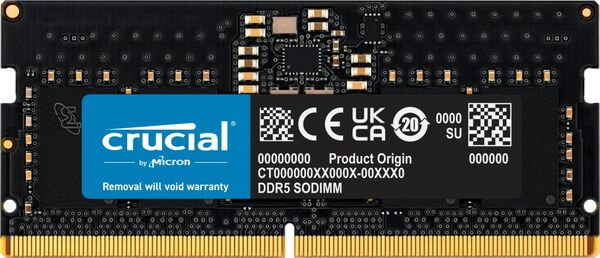
\includegraphics[width=300px]{figures/ram.jpg}
							\caption{RAM modules: DDR5 - laptop}
%				source: https://www.amazon.fr/Crucial-CT8G48C40S5-4800MHz-dordinateur-Portable/dp/B09S2QT75C
					\end{figure}

			\subsubsection{CPU}

				\paragraph{Description}
					Performs base operations (sum, division, etc...) using data stored in memory. Can be described by:
					\begin{enumerate}
							\item Number of cores
							\item Operating frequency, generation, engraving width, supported instructions
							\item \textit{TDP} (W)
							\item Cached memory
							\item \ldots
					\end{enumerate}

				\paragraph{\textit{Multithreading}}
					Idea: perform many tasks simulatneously on a same physical cores \\
					Chez \textit{Intel}: \textit{Hyper-Threading}.
					\begin{equation*}
							\text{\#logical cores} = \text{\#physical cores} \times \frac{\text{\#threads}}{\text{\#physical core}}
					\end{equation*}

				\paragraph{Photos}
					\hspace{1pt}
					\\

					%			sources:
					%			https://m.media-amazon.com/images/I/61Dst+dj-RL._AC_SL1500_.jpg
					%			https://fr.thermaltake.com/toughair-110-cpu-cooler.html
					\begin{figure}[h!]
							\centering
							\begin{tabular}[!h]{c|c}
								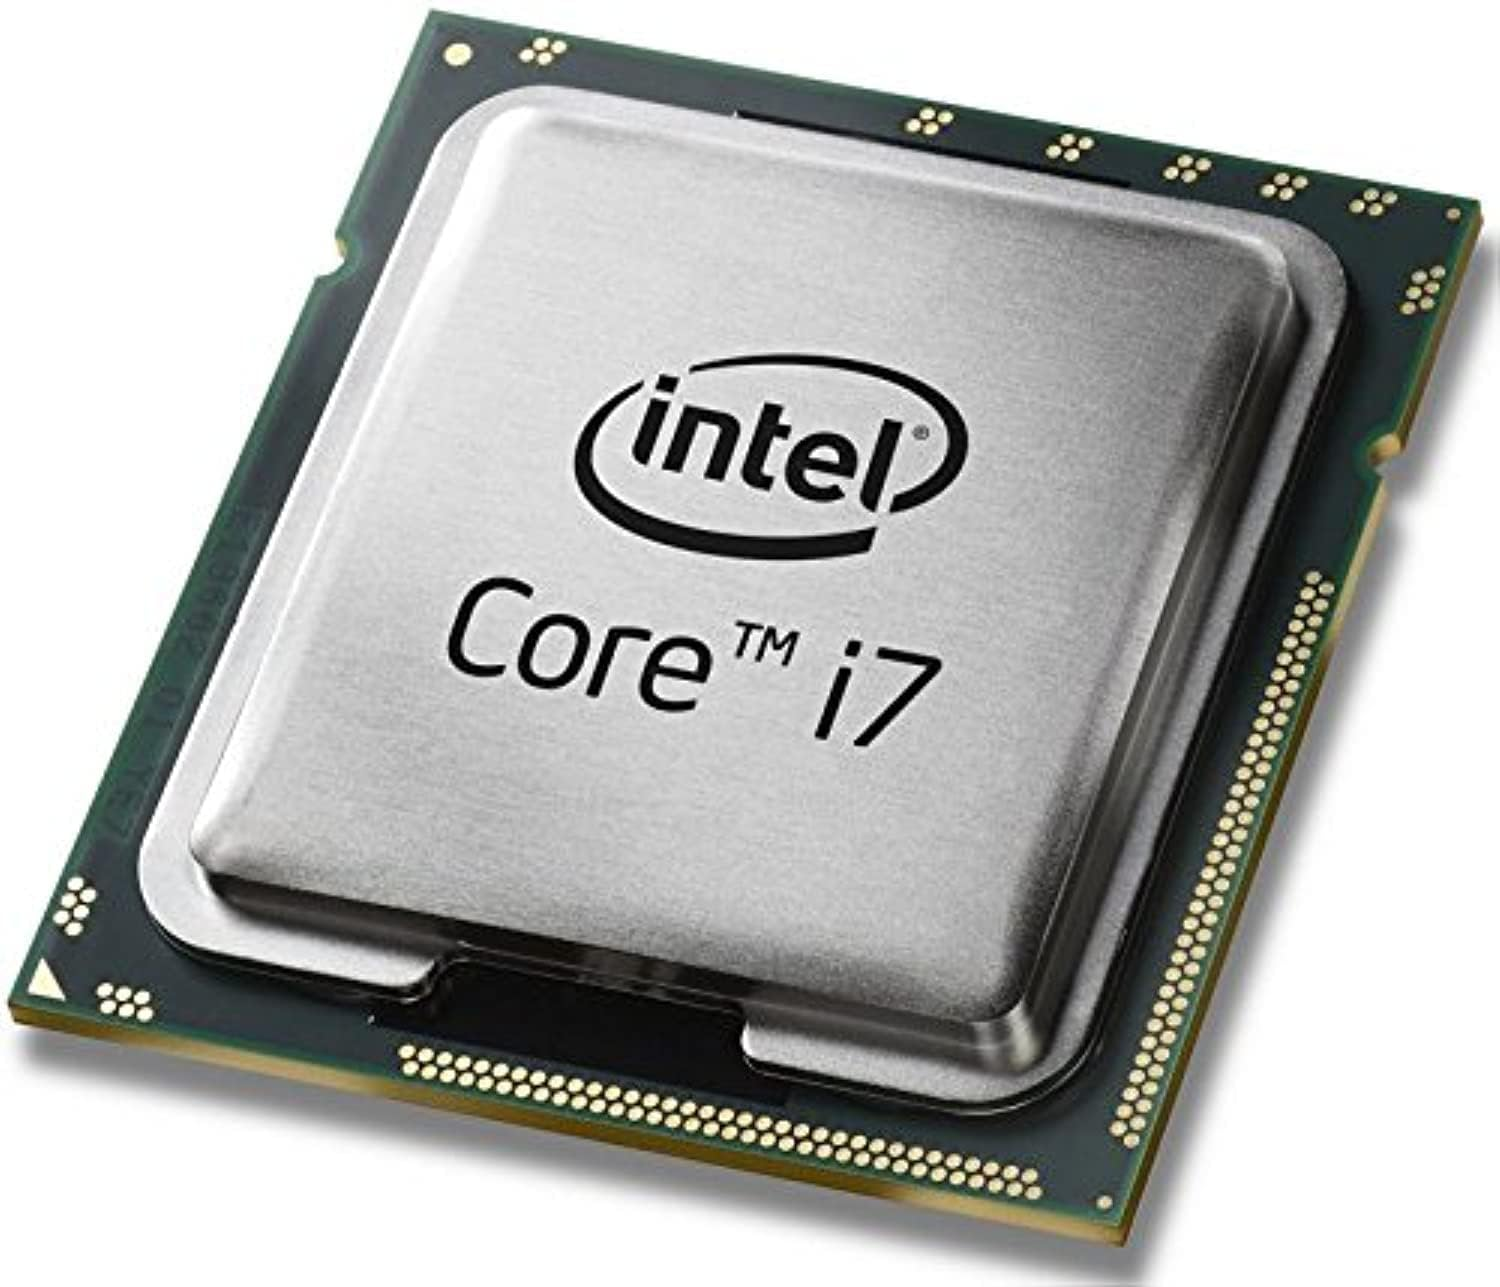
\includegraphics[width=5cm]{figures/CPU.jpg} & 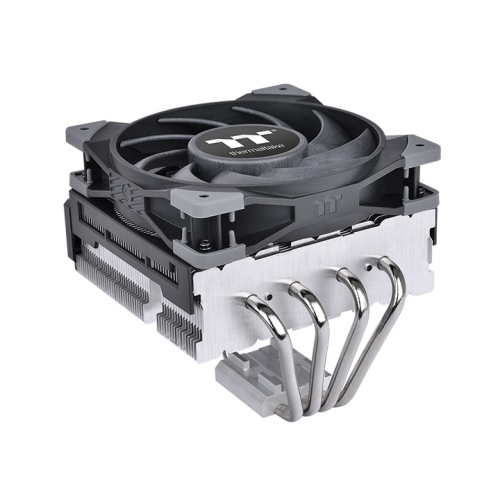
\includegraphics[width=5cm]{figures/CPU_cooler.jpg} \\
								CPU                                          & CPU cooler
							\end{tabular}
							\caption{CPU components}
					\end{figure}

			\subsubsection{Storage}

				\paragraph{Description}
					Save data on the long term. Can be described by:
					\begin{enumerate}
							\item Capacity (GB)
							\item Reading/Writing speed, latency
							\item Type
							\item \ldots
					\end{enumerate}

				\paragraph{Photos}
%					sources:
%					https://www.amazon.fr/Seagate-ST8000AS0002-Archive-HDD-Sata/dp/B00XS423SC
%					https://www.amazon.fr/SanDisk-PLUS-Sata-Internal-Black/dp/B01F9G43WU
%					https://fr.wikipedia.org/wiki/SSD
					\begin{figure}[h!]
							\centering
							\begin{tabular}[!h]{c|c|c}
								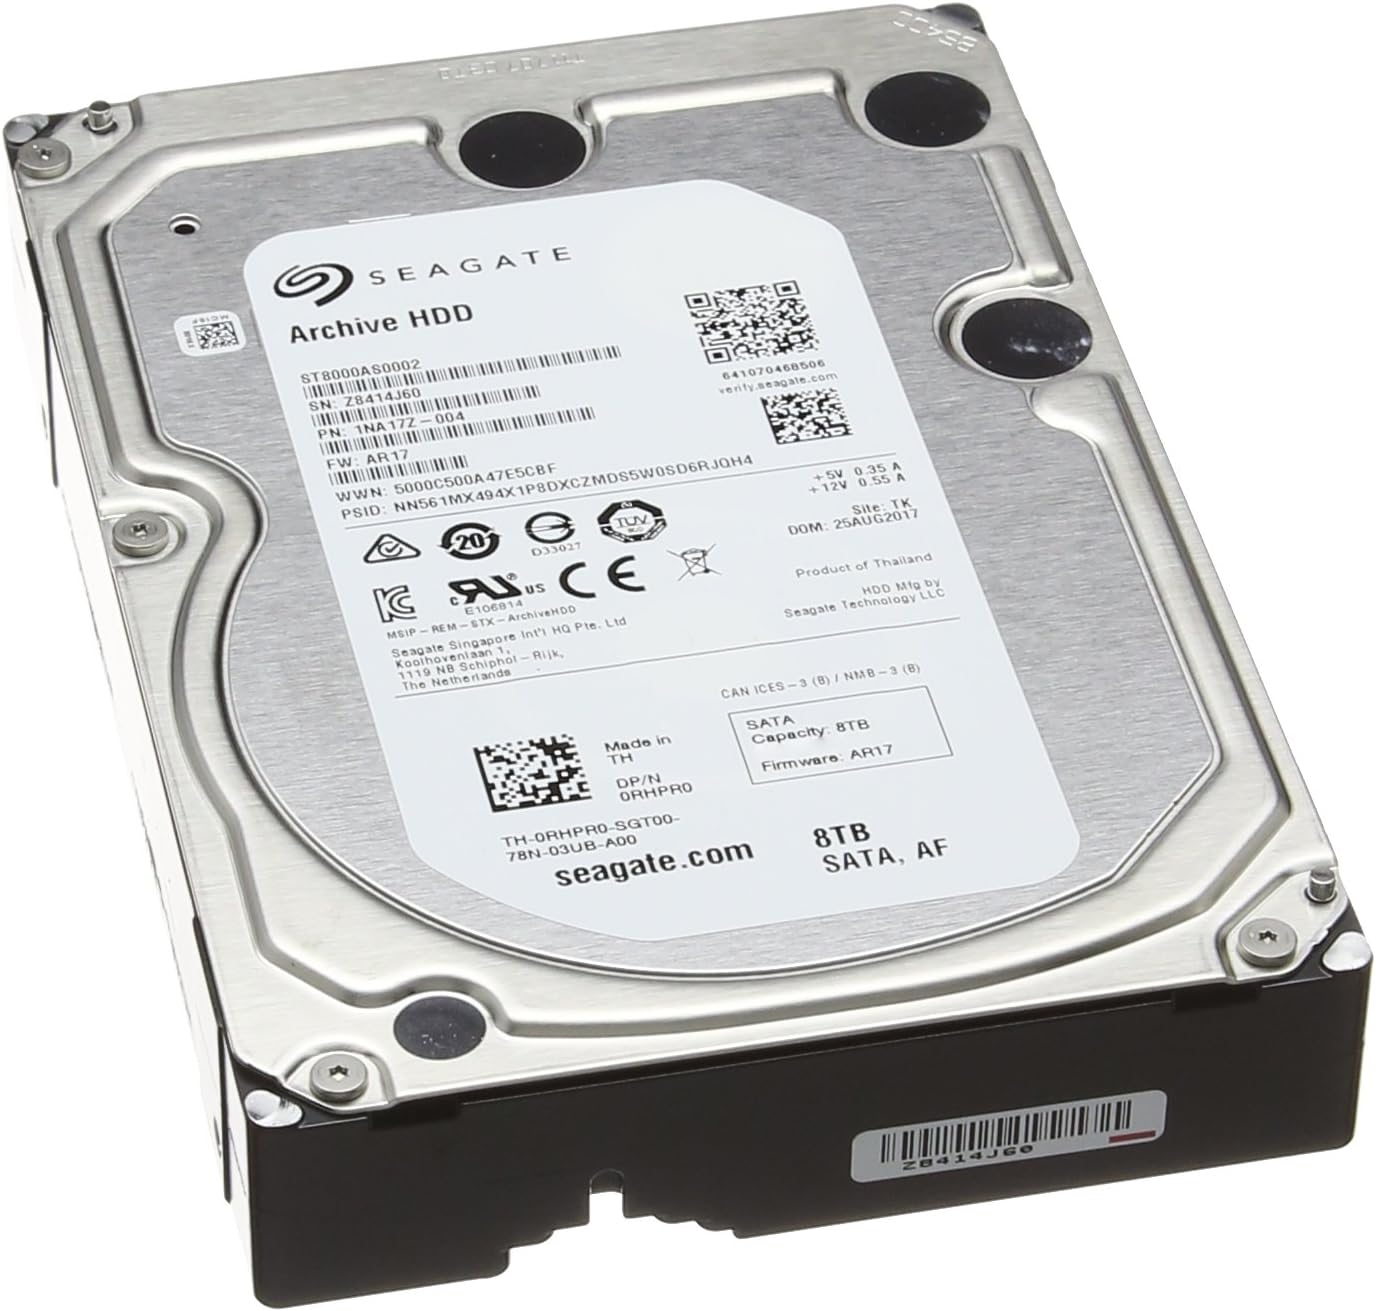
\includegraphics[width=5cm]{figures/HDD.jpg} & 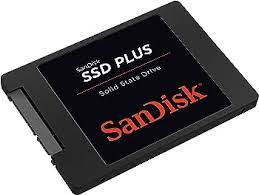
\includegraphics[width=5cm]{figures/SSD.jpeg}
								& 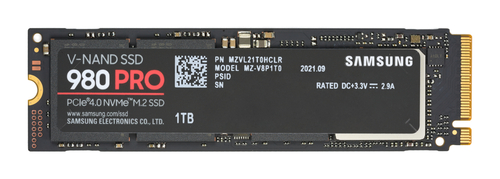
\includegraphics[width=5cm]{figures/M2.jpg}
								\\
								HDD & SSD (old technology) & SSD (new technology)
							\end{tabular}
							\caption{Stockage}
					\end{figure}

			\subsubsection{GPU}

				\paragraph{Description}
					Similar to GPU. Performs graphical operations and produces an image to display 
					More broadly, performs some highly parallelizable tasks. Can be described by:
					\begin{enumerate}
							\item Memory: capacity (GB) and generation (i.e.: frequency)
							\item External connectors
					\end{enumerate}

				\paragraph{GPU and graphic card}
					The word "GPU" describes the computation unit only (not the fans, memory, \ldots).

				\paragraph{Integrated GPU}
					For computers having small graphics needs, the GPU is a small unit dedicated to graphics integrated into the CPU.

				\paragraph{Photos}
%				source: https://www.lesnumeriques.com/carte-graphique/nvidia-geforce-gtx-titan-x-p23635/test.html
					\begin{figure}[!h]
							\centering
							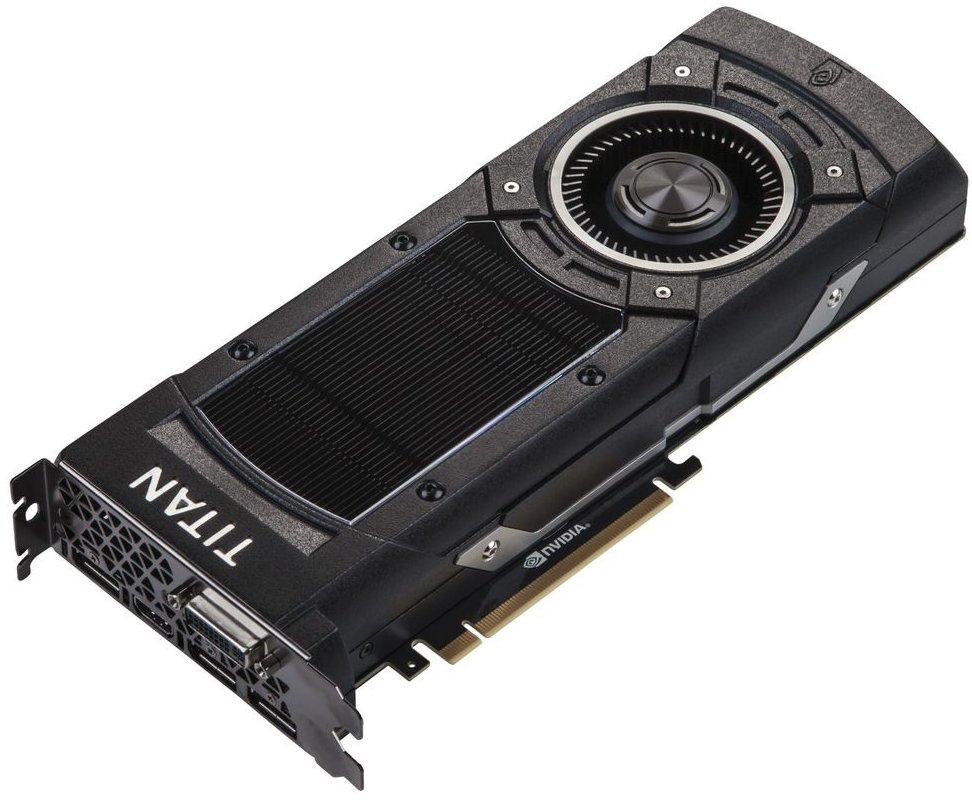
\includegraphics[width=200px]{figures/GPU.jpg}
							\caption{Graphic card}
					\end{figure}

		\subsection{Typical configurations}
			\begin{tabular}{|c|M{4cm}|M{6cm}|}
				\hline
				\multirow{2}{*}{\bf{Component}} & \multicolumn{2}{c|}{\bf{Typical hardware properties}} \\
				\cline{2-3}
				& \bf{Personnal computer}        & \bf{Shared working station}       \\
				\hline
				Memory & 8 GB                              & 64-256 GB                               \\
				\hline
				CPU          & 4-8 logical cores \newline 2GHz & 16-128 logical cores \newline 2-4 GHz \\
				\hline
				Disk         & SSD 500 GB                      & HDD 10 TB \newline SSD 1 TB             \\
				\hline
				GPU          & Integrated                      & 2-8 GB memory                          \\
				\hline
			\end{tabular}

		\subsection{Howto: compare two computers}
			Before any comparison, first ask yourself about the software you want to run:
			\begin{itemize}
				\item Can it be parallelizable?
				\item Is it eunning on GPU or CPU?
				\item Does it need to write or read a lot of data from the disk?
			\end{itemize}
			Two computers can be compared using one of these two methods:
			\begin{itemize}
				\item Compare the date they were bought together with the price at that times
				\item Compare main characteristics:
				\begin{enumerate}
					\item CPU: number of logical cores \\
					(if a GPU exists: generation, memory capacity)
					\item CPU: frequency
					\item RAM: capacity
				\end{enumerate}
				Some websites host a component comparator; typical result is an averaged score built from differents categorical scores (ex: number of cores for a CPU).
			\end{itemize}


	\section{Software}

		\subsection{Operating systems (\textit{OS})}
			An operating system is a software that makes hardware ressources availablethrough interfaces. \\
			We usually make a distinction between low-level component of the OS (e.g.: kernel, handles the hardware) and those that provide
			applications the user can interact with. 

			\subsubsection{Many OS}
				Main OS are:
				\begin{itemize}
					\item Windows (Microsoft)
					\item OS X (Apple)
					\item Linux
				\end{itemize}

			\subsubsection{GUI and CLI}

				\paragraph{\textit{GUI}}: \textit{Graphic User Interface} \\
					Interface that describes software components using drawings. One can interact with a GUI mainly using a mouse.

				\paragraph{\textit{CLI}}: \textit{Command Line Interface} \\
					Interface that describes software components using text. One can interact with a CLI using a keyboard.
					\begin{figure}[!h]
							\centering
							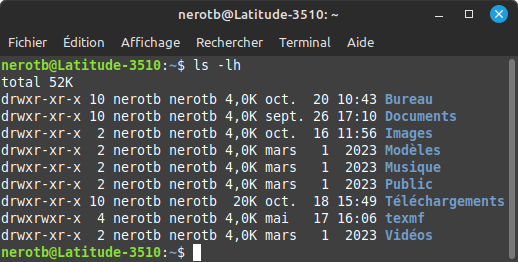
\includegraphics[width=300px]{figures/CLI.png}
							\caption{Linux console (CLI)}
					\end{figure}

				\paragraph{GUI is built on the top of CLI}
					The visual aspect rendered by a GUI is often a simplified version of what can be achieved using the CLI. In the 
					background, most of GUI-related actions are translated to CLI commands at run time.

		\subsection{Processes}
			A process is a set of instructions processed by the hardware as asked by a running software.
			Some processes create several threads that use all the available logical cores. Processes are identified using a
			 \textit{PID} (Process IDentifier).
			\begin{figure}[!h]
				\begin{center}
					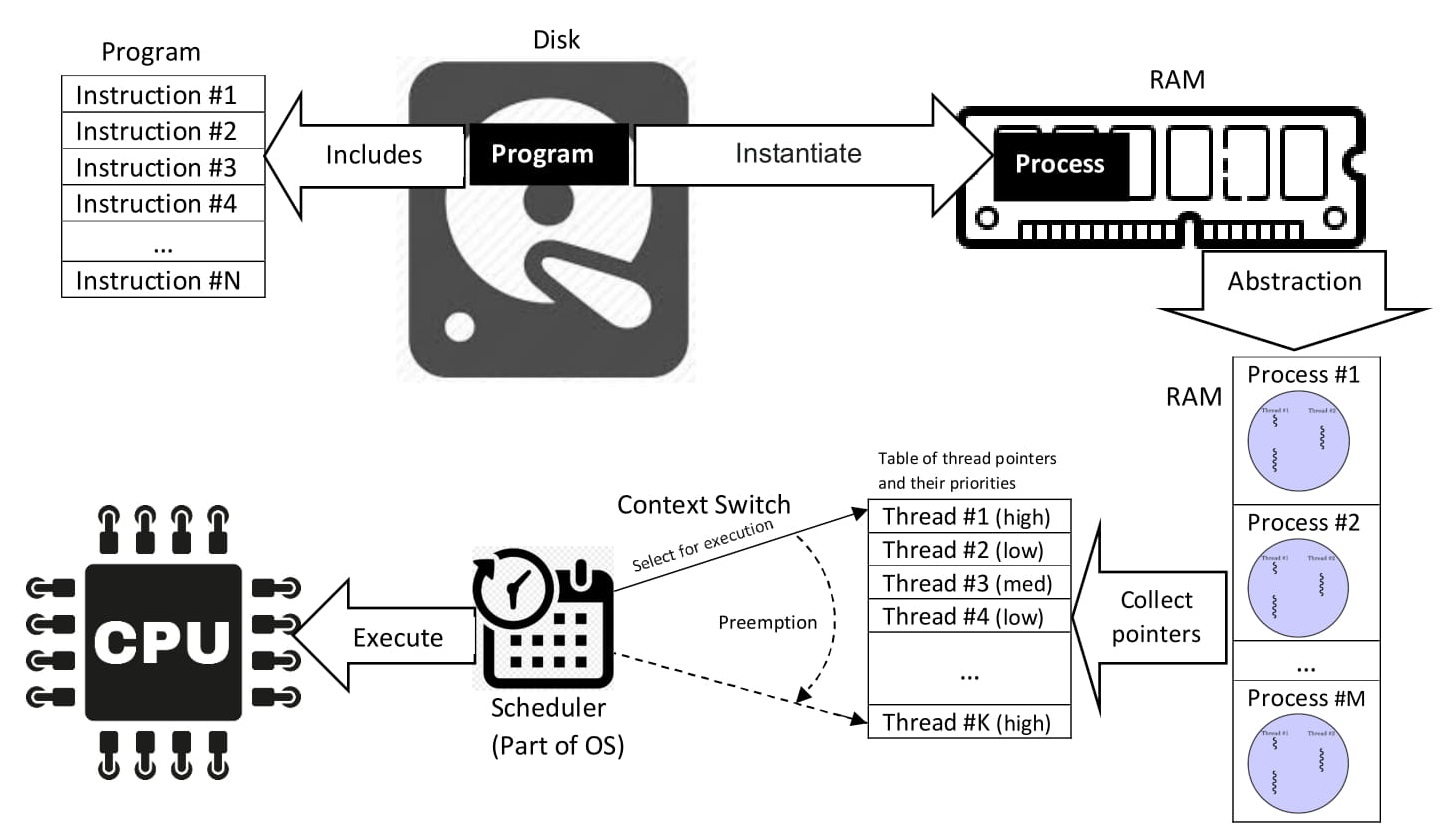
\includegraphics[width=300px]{figures/process.jpg}
					\caption{Simplified running scheme of a software \newline
					\scriptsize{(source: Hooman Mallahzadeh, CC BY-SA 4.0
					\url{https://creativecommons.org/licenses/by-sa/4.0}, via Wikimedia Commons})}
				\end{center}
			\end{figure}

		\subsection{Programing language}
			\begin{quotation}
			[...]
			A programming language is a system of notation for writing computer programs.
			
			A programming language is described by its syntax (form) and semantics (meaning). 
			It gets its basis from formal languages.\\
				\scriptsize{source: Wikipedia}
			\end{quotation}

			\subsubsection{Compiled vs interpretated}

				\paragraph{Compiled language}
					A software written using a compiled language is directly translated into something the OS can handle.
					Examples of compiled languages: Fortran, C++

				\paragraph{interpretated language}
					A software written using an interpreted language is split into pieces
					that make a sense for a master language which handles the execution
					Examples of interpretaed languages: Python, Matlab


\end{document}


%other sources:
%	- https://www.intel.com/content/dam/develop/external/us/en/documents/omg-wp-021609-157200.pdf